\section{Zadanie 1}

\subsection{Charakterystyka metody Hornera}

Metoda Hornera jest techniką stosowaną do szybkiego obliczania wartości wielomianu \( P(x) \) w zadanym punkcie \( x \). Główną zaletą tej metody jest redukcja liczby operacji wymaganych do obliczenia wartości wielomianu, co zmniejsza złożoność obliczeniową z \( O(n^2) \) do \( O(n) \), gdzie \( n \) oznacza stopień wielomianu.

Podstawową ideę algorytmu można przedstawić w następującej formie rekurencyjnej:
\[
P(x) = a_n + x(a_{n-1} + x(a_{n-2} + \dots + x(a_1 + x a_0)))
\]
Dzięki temu każda operacja wymaga jedynie \( n \) mnożeń i \( n \) dodawań, co znacząco zmniejsza czas obliczeń dla dużych stopni wielomianów.

W przeprowadzonych testach dla wielomianów o rozmiarach od 100 do 5000, z krokiem 100, losowano 100 różnych wielomianów dla każdego stopnia. Dla każdego wielomianu mierzono czas obliczenia jego wartości metodą Hornera i standardową, a następnie obliczano średnią z uzyskanych czasów.

\subsection{Wyniki i wnioski}

Poniżej przedstawiono dwa typy wykresów które się pojawiały ilustrujące wyniki eksperymentów:

\begin{center}
\begin{minipage}{0.45\textwidth}
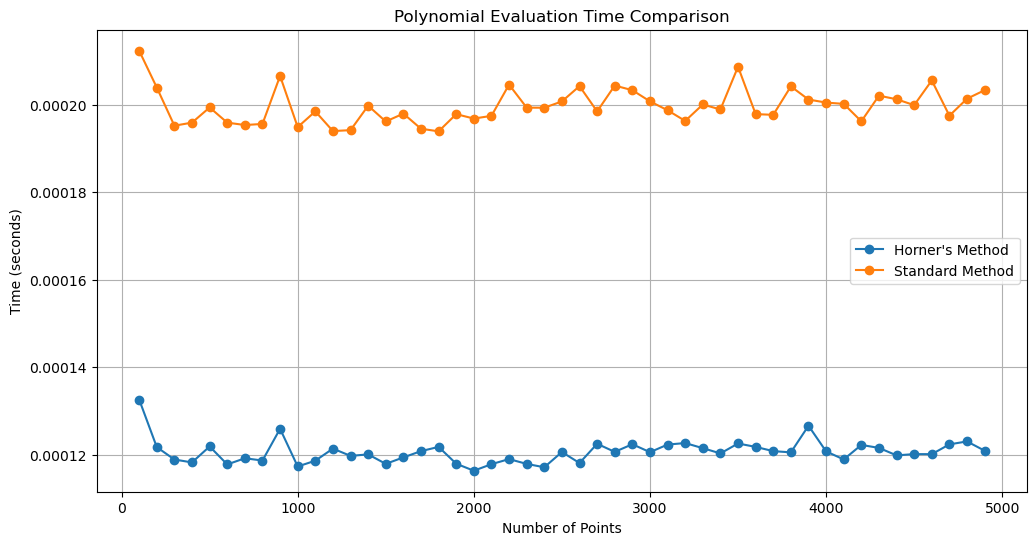
\includegraphics[width=\textwidth]{wykresy/zadanie 1/horner_1.png}
\end{minipage}
\begin{minipage}{0.45\textwidth}
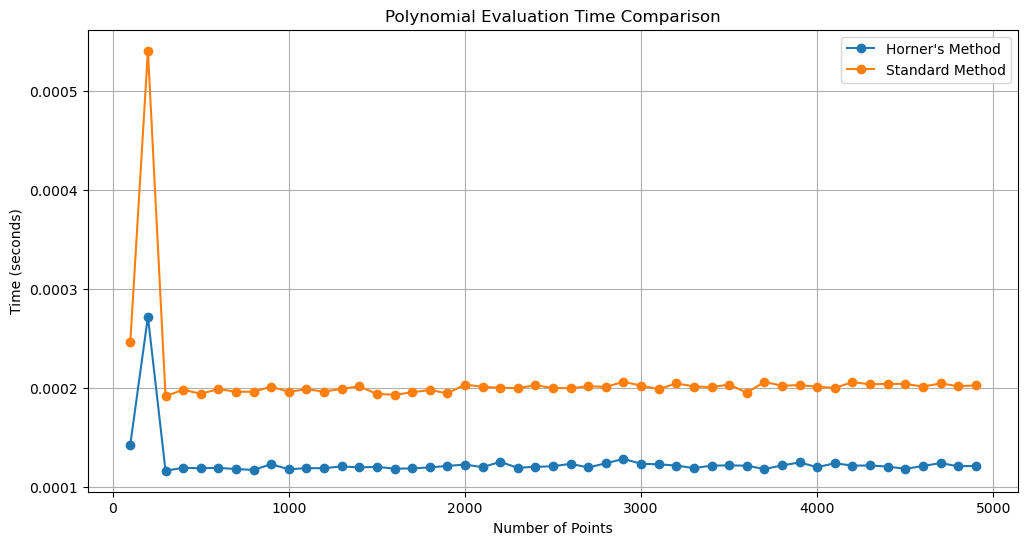
\includegraphics[width=\textwidth]{wykresy/zadanie 1/horner_2.png}
\end{minipage}
\end{center}

\textbf{Wnioski:}
\begin{itemize}
    \item \textbf{Poprawa szybkości algorytmu:} Metoda Hornera pozwala na uzyskanie średniej poprawy szybkości obliczeń na poziomie \( 1.64 \pm 0.04 \). Jest to zgodne z oczekiwaniami wynikającymi ze zmniejszonej złożoności obliczeniowej.
    \item \textbf{Nieoczekiwane skoki czasów:} W niektórych próbach zaobserwowano znaczny wzrost czasu obliczeń dla pojedynczego wielomianu. Zjawisko to nie koreluje z rzędem współczynników ani rozmiarem wielomianu, a jego przyczyna nie jest znana.
    \item \textbf{Skalowalność:} Metoda Hornera wykazuje dobrą skalowalność dla dużych stopni wielomianów, utrzymując stabilny czas obliczeń w porównaniu do klasycznego algorytmu.
\end{itemize}

